


\section{High Energy Physics Applications}

We study applications taken from two experiments of the CERN Large Hadron Collider, namely the ATLAS experiment and the CMS experiment. 
One of the applications of the ATLAS experiment is the \emph{Athena} application, which is a general purpose processing framework including algorithms
for event reconstruction and data reduction \cite{calafiura2005athena}. The CMS experiment is conducted through an application termed  \emph{TauRoast}, which searches for specific 
cases where the Higgs boson decays to two tau leptons~\cite{chatrchyan2013search}. In LHC, the ATLAS and CMS experiments are distinct, 
developed independently by two entirely separate physics communities. Consequently, their applications  
have very different software distribution and data management frameworks, making it interesting to examine if common reproducibility frameworks and 
tools work across the two communities. 


%The application which is the study of this paper is an CMS application~\cite{collaboration2008cms} called \emph{TauRoast}.
%It searches for cases where the Higgs boson decays to two tau leptons~\cite{chatrchyan2013search}.
%Since the tau leptons are very short-lived, they are not observed directly, but by the particle decay products 
%that they generate.  So, the analysis must search for detector
%events that show a signature of decay products compatible with both hadronic tau and top decays.  

Code and data in \emph{TauRoast} is available through five different networked filesystems, namely an HDFS cluster for data files, 
%~\cite{borthakur2008hdfs},~\cite{sandberg1985design},\cite{welch2008scalable}, ~\cite{howard1988scale}
some configuration files were stored on a CVMFS~\cite{blomer2011cernvm} filesystem, and a variety of software tools were on an NFS, PanFS and AFS systems.
In addition, code may exist in version control systems such as Git, CVS, and CMS Software Distribution (CMSSW). %~\cite{cms2006cms}. 
\begin{wrapfigure}{r}{0.4\textwidth}
\small
\centering
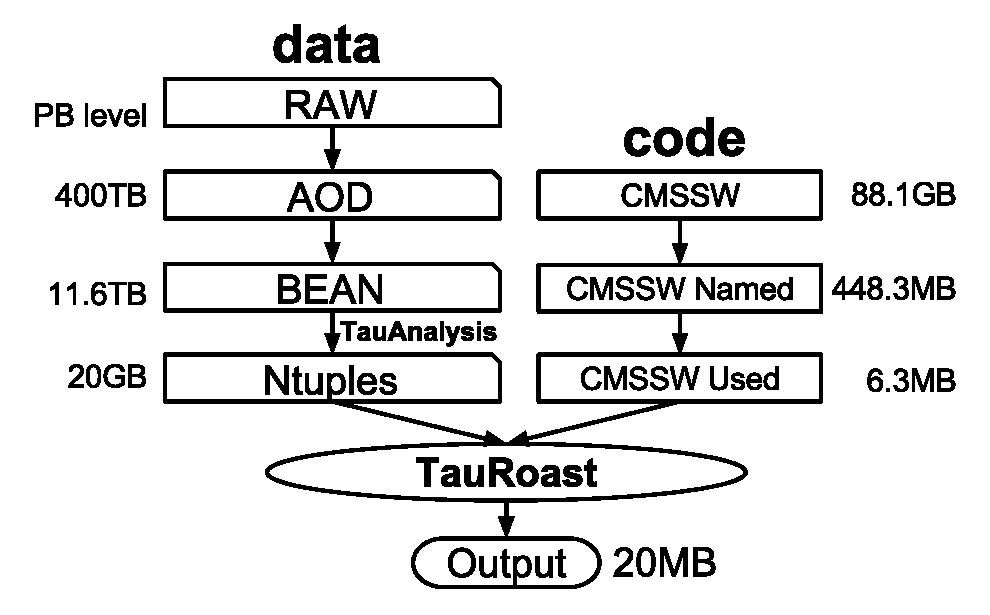
\includegraphics[width=.4\textwidth]{data-code-size.eps}
\caption{Inputs to Tau Roast}
\label{fig:data-code-size}
\end{wrapfigure}
Data that is input to \emph{TauRoast} is obtained by reducing it through a pipeline, as shown in Figure \ref{fig:data-code-size}. Consequently, the real input data may 
vary depending upon the science question being researched. Similarly the software may name many possible components but the used components are
smaller than the named ones. 

In \emph{Athena} data is obtained through an external Dropbox-like system called the FaxBox, but does not go through any reduction steps. Code is obtained through 
CVMFS, which provides the analysis routines. However, depending upon the input data code and the configuration that will be invoked changes. 
Thus in \emph{Athena} the used code and configuration are dynamic depending upon input data, where as in \emph{TauRoast} the code and data are static, 
but the amount of data and code to include changes depending on the involved science. 


%In application, code and data that form the applications are drawn from large external repositories through multiple step reductions. 
%Figure \ref{fg:data-code-size} shows the data and code reduction and reliance on software distribution repositories. There are two observations to be 
%derived from 
%of this reduction. First. the actual code contributed by individual groups, in this case the CMS and ATLAS group, is small. 
%But the contributed software relies on several software dependencies, which
%are available software distribution repositories such as the CMS Software Distribution (CMSSW)~\cite{cms2006cms}, and the CVMFS. 
%These repositories contain many different tools, libraries, and utilities, and for ATLAS, the Reco\_TR analysis framework which consists of many analysis routines. 
%
%Figure~\ref{fig:data-code-size} shows that both the code and data
%that form \emph{TauRoast} are drawn from large repositories through
%multiple steps of reduction.  A preservation strategy must weigh
%whether to store the large repositories completely, the fragments
%used by an artifact, or something in between.
%
%{\bf Code Sources.} Like many scientific codes, the central algorithm
%of \emph{TauRoast} is expressed in a relatively small amount of
%custom code developed by the primary author.  But, the code cannot
%run at all without making use of an enormous collection of software
%dependencies.  
%The largest of these repositories is the CMS Software Distribution (CMSSW)~\cite{cms2006cms},
%which contains many different tools, libraries, and utilities.  No single code uses anywhere close to all of these.  But, because it is widely used within the experimental researchers, it is common for users to simply expect that a particular version of the entire repository is available.
% 
%{\bf Data Sources.}
%The CMS collaboration provides end-users with a pre-processed
%and reduced data format, AOD~\cite{holtman2001cms}, 
%which is based on the RAW output of the CMS detector readout electronics and reconstructed world-wide.
%As AOD data are too large to be iteratively processed repetitively in
%a physics analysis workflow, it is normally reduced further in
%structural complexity and content.  For the analysis under
%investigation here, this is a two-step process.  First, the AOD data
%are processed at the Notre Dame working group cluster to BEAN (Boson Exploration Analysis Ntuple) events,
%containing only trivial data containers packed in vectors.  This step
%is time and CPU intensive and its output contains data of 11.6$\,$TB to be
%analyzed by the tau analysis.
%In the second step, the data are reduced to the ``Ntuple'' format,
%which contains only events matching basic quality criteria and
%fields relevant to \emph{TauRoast}.
%Once the data has been reduced to Ntuples, TauRoast can be run as a single
%process, and contains a stringent event selection to look only at high
%quality candidate events for the underlying physical process.
%Quantities from the relevant events can be
%both plotted and used in multivariate analysis to determine the level
%of expected signal in real data.

